\section{Current contributions}

\subsection{Proof of Concept}

\begin{figure}[!b]
   \begin{center}
      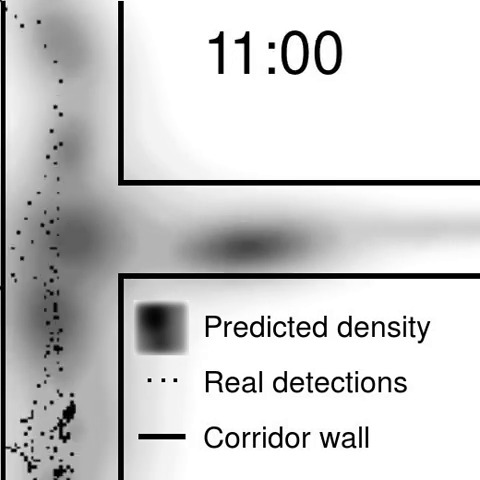
\includegraphics[width=0.3\columnwidth]{fig/corridor_0}
    \hfill
      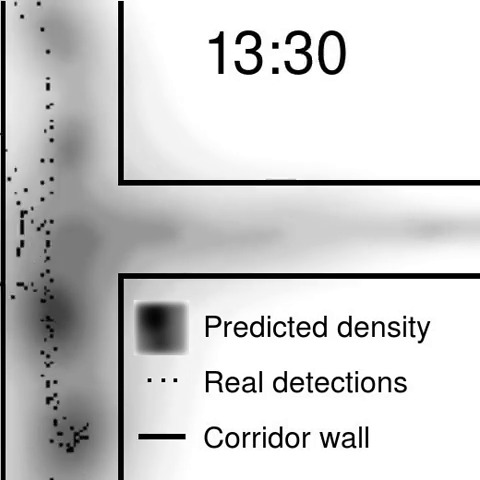
\includegraphics[width=0.3\columnwidth]{fig/corridor_1}\\\vspace{5mm}
      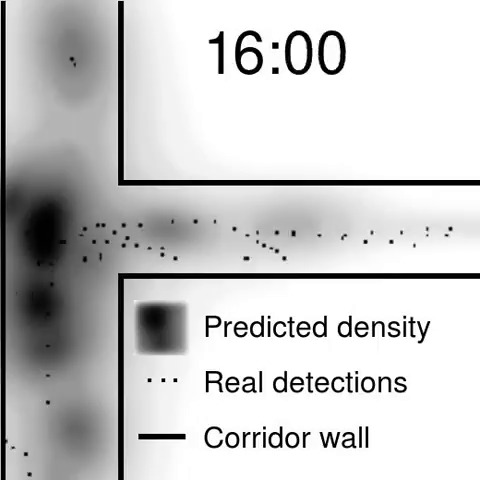
\includegraphics[width=0.3\columnwidth]{fig/corridor_2}
    \hfill
      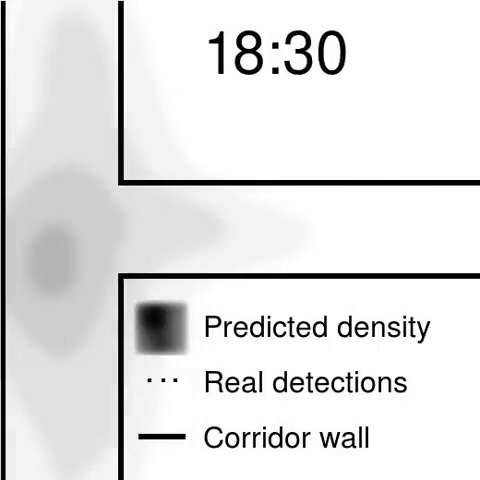
\includegraphics[width=0.3\columnwidth]{fig/corridor_3}
      \caption{Screen grab from the video available at~\url{https://youtu.be/4SW4j7DDxYE}.\label{fig:video}}
   \end{center}
\end{figure}




\begin{itemize}
    \item T.~Vintr, S.~Molina, J.~Fentanes, G.~Cielniak, T.~Duckett, and T.~Krajn{\'i}k, ``Spatio-temporal models for motion planning in human-populated environments,'' in \emph{Student Conference on Planning in Artificial Intelligence and Robotics}, 2017.
\end{itemize}

In \cite{vintr2017spatiotemporal} we proposed a concept of modelling human activities over the time in their natural environment.
We hypothesised that there are some patterns of human behaviour over the timeline.
As these patterns are derived from the routines and habits of humans, these patterns show periodical and continuous nature.
We also hypothesised that there are no or negligible trends in these patterns due to the nature of human habits. 
Let us consider these examples to explain periodicity and continuity of human behaviour:

... copy from mesas ...
\begin{itemize}
    \item the human  behaviour is very similar during every morning as opposed to the difference in behaviour during morning and afternoon of one randomly chosen day,
    \item human behaviour five minutes before midnight and five minutes after midnight could be probably very similar, although we compare behaviour in two different days,
    \item contrary to that, human behaviour during Sunday afternoon is probably different from behaviour on Monday afternoon.
\end{itemize}
... end ...

Such a periodical behaviour is not only forced by natural physical demands like fatigue or hunger, but also by social demands like regular working hours or the compulsory education system. 

To create the model of the time-dependent patterns of human behaviour, we need to estimate the parameters of their distribution.
As the timeline is continuous and it is not possible to repeat the experiment at the same time, the timeline is not suitable as a domain for time-dependent feature parameters estimation, especially for rare events.
The conventional approach to this task, known as time series forecasting, is to divide time-dependent events into three different components - a trend, seasonal and cyclic patterns - and analyse them separately \cite{gould2008forecasting}.
The cyclic patterns are not predictable changes in the time series, seasonal patterns are the periodical changes, and the trend is continuous growth or decrease of measured values.
To model human behaviour with the assumption of high periodicity and no trend, but with the accent to the continuity, we not only find and model dominant periodicities but also project timeline into the new multidimensional vector space.
In particular, we project every chosen periodicity into the $2d$ circle in the way, that every pattern that occurs periodically and matching chosen periodicity projects in the same position in this circle.
By this projection we solve two issues:
\begin{itemize}
    \item the time domain is constrained, and therefore it is possible to estimate distribution parameters of the time-dependent periodical patterns,
    \item and the continuity is guaranteed.
\end{itemize}

\subsubsection{Time Projection in Detail}

To prove this concept we used data of human positions during two days collected at the corridors of the School of Computer Science at the University of Lincoln.

... copy from pair ...
Data collection was performed by a mobile robot equipped with a Velodyne 3d laser range-finder.
The robot was placed at a T-shaped junction so that its laser range-finder was able to scan the three connecting corridors simultaneously.
To detect and localise people in the 3d point clouds provided by the scanner, we used an efficient and reliable person detection method~\cite{yan2017online}.
Each day contains approximately $28000$ entries, which correspond to hundreds of people walking or standing in the monitored corridors.
... end ...

The dataset consists of vectors $\left(x, y, t\right)$.
For the sake of simplicity we chose only one periodicity $T = 86400 s$ (one day), and project these vectors into the extended vector space in this way: $\left(x, y, t\right) \rightarrow \left(x, y, \cos\frac{2\pi t}{T}, \sin\frac{2\pi t}{T}\right)$.
Then we modelled the distribution by the Gustafson--Kessel Algorithm~\cite{gustafson1979fuzzy} with the number of clusters $k=30$.

We visualised this model of "distribution" of people at corridors in the form of a video that can be found online at [nechunkcni odkaz].
Every video frame, Figure~\ref{fig:video}, consists of $5$ minutes time frame reconstruction and the whole video consists of two days.
We can see that the model changes over time and respects corridor boundaries. 

